\pdfoutput=1

\documentclass{l4proj}
\usepackage{comment}
\usepackage{graphicx}
\usepackage{caption}
\usepackage{url}
\usepackage{bytefield}
\usepackage{color}
\usepackage{tikz}
\usepackage{hyperref}

%
% put any packages here
%

\DeclareGraphicsRule{.1}{mps}{*}{}
\begin{document}
\title{Designing a lightweight protocol for constrained devices for use in the Internet of Things paradigm}
\author{Dr. Fergus W. Leahy}
\date{\today}
\maketitle

\begin{abstract}
\textbf{PLACEHOLDER}
A level 4 project which explores the current use of protocols for the Internet of things devices.
\end{abstract}

\educationalconsent
%
%NOTE: if you include the educationalconsent (above) and your project is graded an A then
%      it may be entered in the CS Hall of Fame
%
\tableofcontents
%==============================================================================

\chapter{Introduction}
\pagenumbering{arabic}
The ``Internet of Things'' paradigm, along with the ``Smart'' prefix, has recently seen a significant rise in interest and popularity with manufacturers, hobbyists and end-users. Everything from your set-top box to your washing machine can now be ``Smart'' and connect to the Internet to tell you if your favourite TV show has downloaded or that your wash cycle has complete\cite{LG, SmartCraze}. Some hobbyists have gone so far as to make a plant send a text or tweet when it needs watering\cite{Botanicalls, TweetPlant}.

This uptake in interest and development can be largely attributed to the advent of lower power, smaller and cheaper devices. Large companies, such as the mobile phone chip-set manufacturer Qualcomm, recently declared their support at CES 2012 with the announcement of a dedicated development platform for the ``Internet of Things''\cite{Qualcomm}.

Similarly there has also been much enthusiasm from small companies and start-ups trying to create the next hit consumer device. The social funding platform, Kickstarter\cite{Kickstarter}, has seen many attempts at creating the perfect ``Thing'' for the Internet\cite{SmartThings, Twine}.

Whilst all of these devices from manufacturers, start-ups and hobbyists may very well be great ``Things'' by themselves, there exists a problem. How does one connect all of these heterogeneous platforms and devices together to create a truely interconnected ``Internet of Things''?

This project focuses on just that and endeavours to create a communication protocol that is not only platform agnostic but also lightweight enough to be run on the most constrained devices, such as the TelosB Sky Motes(8MHz CPU,10K ram)\cite{TelosB}. Another core design focus is that the protocol must be able to scale effectively as the network dramatically increases size as can be expected with the rapidly increasing availability of network-connected devices.
%==============================================================================
\chapter{Background and Related Work} % (fold)
\label{cha:background}
\section{What is the ``Internet of Things''} % (fold)
\label{sec:internet_of_things_paradigm}
This section describes the concept of the ``Internet of Things'', its slow development up to the present, and the motivations as to why one would want to create an ``Internet of Things''.

\subsection{Past, Present and Future} % (fold)
\label{sub:past_present_and_future}

% subsection past_present_and_future (end)
The standard model of how we use computers and the Internet today revolves around the idea of an interconnected network of servers, routers and data centres around which users connect using their personal computers to access, input, manipulate and retrieve data. 

This model heavily relies upon the users to provide the data from which the Internet is powered. Without this data the Internet would be a barren place, with nothing to search for, sell, buy, share, watch, listen to, play, analyse or learn from.
Users from all around the world have contributed to make the Internet \textit{the} single biggest resource in the world by snapping photos, capturing videos, writing blogs, creating websites, commenting, discussing, reviewing, buying, selling and inputting data. So much data in fact that the estimated size of the Internet in 2009 was 500 exabytes (that's 500 BILLION gigabytes), of which 70\% was contributed to by users.\cite{Size}   

% INSERT DIAGRAM HERE
Within this model there exists two significant problems posed by users; time and accuracy. In terms of time, users only have so many hours in a day to input data; which can only be so accurate, as all users are prone to error through one means or another.
These two problems make it difficult to observe our world and represent it in an accurate and reliable digital form.

The idea of taking this responsibility of inputting data away from the user and giving it to the machine is where the ``Internet of Things'' term initially came from. The term itself was thought to have first been coined by Kevin Ashton\cite{K.Ashton} in 1999, who at the time was interested in linking up a company's supply chain to the Internet using RFID technology to allow for autonomously monitoring its state.
Sadly, at that time the idea progressed little and didn't garner much support.

Fast forward to 2013, the ``Year of the Internet of Things'' as declared by the MIT Technology Review\cite{2013IoT} and observed in the Consumer Electronics Show 2013 (CES) with manufacturers introducing everything from smart fridges to smart weighing scales. Concurrently, low power devices have become increasingly affordable and small enough to embed into other devices, making it much more possible to create a truly autonomous system, either in the home, office or car, wherein the user doesn't have to interact directly with any of the devices but instead just go about daily life, which, in the background, is enhanced by these ubiquitous devices operating together.

With all the possible ``Things'' that can exist, the core functionality in the ``Internet of Things'' can be simply modelled as closed loop system in which a ``Thing'' can sense, process and interact with the real world as well as other devices and services. This system is represented at its simplest by an if statement, \textit{if \textbf{event occurs} then \textbf{do action}}, which provides developers and users alike an easy to understand yet powerful model to create rules for autonomous interaction.i.e.
\begin{center}
	\textit{if \textbf{temp \textless  20C} then \textbf{Turn ON heating}}

	\textit{if \textbf{washing machine done} then \textbf{Text John}}
\end{center}

There currently exists a variety of online services and devices which give the end-user this ability to do such tasks, such as the Twine device \cite{Twine} which is a small low power device with a variety of sensors and a WI-FI radio. The goal of the device was to make it simple and easy to set up and use; the user just puts the device in the desired environment, perhaps on a washing machine, sets up some rules (``When accelerometer is knocked Then tweet''), and when the condition is true, the preset action, in this case tweeting, is performed. Whilst this gives the user great flexibility to perform actions automatically, the limitations show when trying to interact with more than one Twine or with other devices and not just Internet services. 

\begin{figure}[h]
	\centering
	\begin{minipage}{.5\textwidth}
		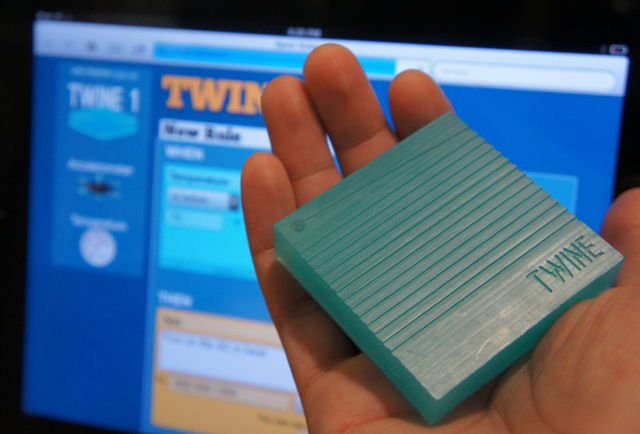
\includegraphics[width=.6\linewidth]{images/twine-device.jpg}
		\captionof{figure}{Twine IoT device.}
		\label{fig:twine_device}
	\end{minipage}%
	\begin{minipage}{.5\textwidth}
		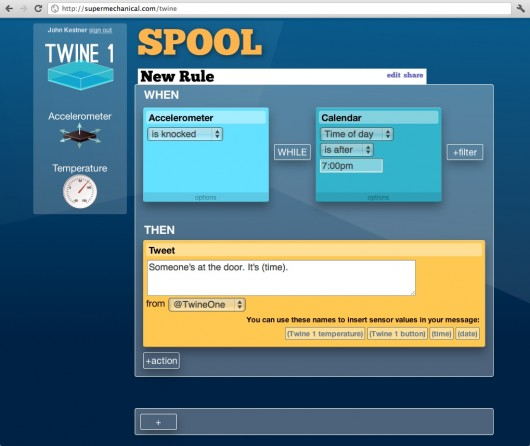
\includegraphics[width=.6\linewidth]{images/twine-rules.jpg}
		\captionof{figure}{Twine rule, When x Then y}
	\end{minipage}
\end{figure}

The Twine device isn't the only device out there, Smart Things\cite{SmartThings} goes one step further than Twine and gives the user a network of devices connected to the Internet through a central hub which the user can then interact with online.

The main problem that exists and will continue to do so is that the digital environment is filled with a huge variety of heterogeneous devices; the key to the future of the ``Internet of Things'' is to find a way to abstract away the differences between these devices and create a simple platform on which all types of devices can communicate to build a more rich and powerful ``Internet of Things''.
\newpage
\subsection{Motivation} % (fold)
\label{sub:motivation}
Like any new paradigm of computing, there must be sufficient motivation and interest for it to be picked up, used and developed further. In the case of the ``Internet of Things'', there are many cases why such a paradigm is of great interest, both to consumers and organisations.

\begin{itemize}
	\item Workload 
	\begin{itemize}
		\item As mentioned previously, the core principle of the ``Internet of Things'' is to stop the user from having to consciously input data into systems, instead, replacing them with new devices(sensors, actuators). By doing so, the user's workload is reduced, giving them more time to do other activities, either of more interest or importance. 
	\end{itemize}
	\item Cost and Eco-savings
	\begin{itemize}
		\item One of the key benefits from collecting data from these devices rather than users is that more accurate and reliable data can be gathered, from which smarter decisions can be made for the user, often resulting in energy savings i.e, turning off unnecessary lights or optimising heating schedules. These energy savings not only benefit the user in terms of monetary cost but also benefit the planet, making it valuable to both the individual and larger community as a whole.
	\end{itemize}
	\item Security
	\begin{itemize}
		\item By utilising these devices, not only can data be collected reliably but actions can also be executed reliably, unlike users. This can benefit the user in terms of security, ensuring that an important action is always carried out i.e, automatic door and windows locking upon exiting the house.
	\end{itemize}
	\item Remote
	\begin{itemize}
		\item Because of the connectivity of these devices, users can interact with them from anywhere with an Internet connection, giving them access to change, update and ensure the system is working correctly i.e, check oven is turned off and front door locked when out.
	\end{itemize}
\end{itemize}


% Reducing work load giving people back more time, simplifying life
% Improving security, 
% ECO
% COST SAVING
% Improving living standards

% subsection motivation (end)

\section{Typical ``Internet of Things'' examples} % (fold)
\label{sec:typical_}
In order to better understand the possibilities and typical scenarios surrounding an ``Internet of Things'' equipped home or office, this section will outline two ideal examples of an ``Internet of Things'' network embedded in the home and office, discuss their respective benefits as well as the current state of ``Internet of Things'' networks.

\subsection{``Internet of Things'' at Home} % (fold)
\label{sub:home}
The most common association with the ``Internet of Things'' is the ``Home of the Future'', which gives the consumer the impression that the static home they are used to will come alive with technology, to make life at home far simpler and more enjoyable. Therefore, this initial example will focus on the ``Internet of Things'' around the home and demonstrate several uses of it.

The primary goal of an ``Internet of Things'' network embedded in the home is to create an awareness of the user. By making the home aware of the user, it can observe them in real-time and determine \textit{smart} things to do autonomously within the home. These could relate to security, such as locking and unlocking doors and windows when the user enters or leaves, or relate to convenience, such as turning on and off appropriate lights as the user moves between rooms, turning on the heating in anticipation of the user's arrival. 
Over longer periods of time it could keep track of the user's habits and adapt heating schedules or open the blinds when the user usually goes to sleep or wakes, it could even turn on the coffee pot so when the user awakes in the morning a fresh cup of coffee awaits them.

Other examples are less concerned with the user but instead with the safety and upkeep of the home, by embedding sensors within objects in the home autonomous maintenance can be carried out. Some examples of this could be, automatic plant watering when low soil moisture is detected, or autonomous vacuuming at certain periods of time when the user is away.\cite{Roomba} By creating these possibilities, it not only reduces the workload for the user but it also allows the user to do things which matter most to them, and of course it stops plants from being forgotten about.

\subsection{``Internet of Things'' at Work} % (fold)
\label{sub:work}
Much of the benefits from deploying an ``Internet of Things'' at home also apply when deployed in a work environment, such as energy savings, reducing workload and increasing security.

In the workplace, the concept of the ``Internet of Things'' being aware of the user could be taken advantage of to a much greater extent to increase productivity, efficiency and independence. This could be possible by allowing workers to be automatically checked in and out of their office and other key locations within the workplace, such as the cafeteria or meeting rooms, with varying granularity based on privacy. By doing so, not only can a worker forget about informing colleagues of their location through punch cards or switchboards, but it can also help keep their colleagues to be more informed about each other, so that instead of finding an empty office after walking from the other side of the building, time can be better spent.

% subsection  (end)
%  home (end)


% subsection typical_ (end)
 % Kevin Ashton, RFID, coined IoT
 % http://www.rfidjournal.com/article/view/4986
 % Giving everyday objects a digital presence and creating machine to machine connections
 % Autonomy, semi-autonomy
 % Taking the human out of the equation and empowering the computer to produce and consume its own data to make our world more 
 % efficient, less wasteful, more time and less energy.
 % Slow start, not much going on.

 % 2012/13 jump start, lots of manufacturers
 % open hardware initiatives
 % linking home automation, security and IoT i.e. toaster/coffee machine
 % 

 %%%%%%%%%%%%%%%%%%%%%%%%%%%%%%%%%%%%%%%%%%%%%%
% HOME AUTOMATION? ??????????????????????
%%%%%%%%%%%%%%%%%%%%%%%%%%%%%%%%%%%%%%%%%%%%%%%%%%


% section internet_of_things_paradigm (end)
\newpage
\section{Open source constrained devices} % (fold)
\label{sec:open_source_constrained_devices}

In the past 5-10 years, there have been many attempts at creating an affordable, low power and approachable electronics platform such as Arduino, Netduino, BeagleBone, Teensy and MSP430 Launchpad. All of which have taken very different approaches, some opting for absolute low cost (MSP430 Launchpad), whilst others aimed to be fully featured and powerful devices (BeagleBone). Other devices such as the TelosB mote, whilst not cheap, has fuelled academic research into new ways of designing and implementing Wireless Sensor Networks. More recently, the Raspberry Pi has created a whole new market of super, low-cost, yet moderately-powerful computers aimed at education and hobbyists.

In the rest of this section a variety of different devices and platforms will be discussed including the Arduino, TelosB mote, Raspberry Pi and other ``Internet of Things'' related devices. 

\subsection{Arduino} % (fold)
\label{sub:arduino}

The Arduino was born in 2005 at an Italian university, Interaction Design Institute Ivrea, out of the necessity of creating a cheap and approachable electronics platform which could enable design students to create interaction design projects without the need of an electronics background.
The main device which was created and has remained much the same since, is based on an Amtel ATmega328 8bit micro-controller running at 16MHz with 2KB of RAM and 32KB of storage for programmes written in a variation of C/C++. The board itself maps out the micro-controller's mix of 20 digital and analogue input/output pins and supports several standardised protocols for communicating with other devices such as I\textsuperscript{2}C\footnote{I\textsuperscript{2}C - Inter-Integrated Circuit} and UART\footnote{UART - Universal Asynchronous Reciever/Transmitter}. 

But the key to the Arduino Platform is not the micro-controller itself but instead the design, software and support provided by the creators and other developers. The other major factor to its success is that the device, along with the documentation and support, are all open source, thus allowing anyone to learn from, replicate and expand upon the platform in any way they wish.

An example of how these factors have had a hugely positive effect is something which Arduino calls ``Shields''. These shields plug in on top of the Arduino board and contain standard components which can add additional features such as WI-FI, Ethernet, sound, motor control etc. Rather than users being required to find, purchase and solder the required components to add such features, these pre-built shields provide it in simple and readily available package, made by a variety of manufacturers.

Since its creation, the Arduino platform has created a range of Arduino named devices and shields resulting in a following of over 300,000 users\cite{ArduinoNumbers} and support from many manufacturers and distributors worldwide. 

Due to Arduino's open source licensing policy, many new start-ups have been able to quickly design prototypes and products using the Arduino platform which have been taken to market in various refined forms. Often the same micro-controller which powers the Arduino is kept and the board miniaturised to fit the product's needs. Products such as the Internet ``Thing'' Twine\cite{Twine} and the Smart Things ``Internet of Things'' eco-system have taken this approach\cite{SmartThings}.

However, whilst there is an abundance of Arduino devices in the wild with many being used as an Internet ``Thing'', there is yet to be created an open and compatible method to easily network a group of such devices together to form a connected ``Internet of Things'' network.

\begin{comment}
OPEN SOURCE
Micro-controller, cheap, easy, PIC chips were difficult, lowered barrier of entry, provided large support and huge following
Italian made, several iterations on size and power
Good starting point for development as there are many in existence
Well adopted
Based on C/C++ with a few tweaks, offers shields for expandability i.e. Ethernet, WI-FI
very good at sensing and doing things
16MHz
no threading
\end{comment}
% subsection Arduino (end)

\newpage
\subsection{Raspberry Pi} % (fold)
\label{sub:raspberry_pi}
Launched in 2012 the Raspberry Pi, a \$35 credit card sized computer, was eagerly anticipated to change the computing landscape. The charity behind it, the Raspberry Pi foundation, had one main goal; to refresh and promote the teaching of computer science in schools.

Similar to the Arduino Platform, most of the hardware and software for the device is open source with the aim of letting adults and children alike get their hands dirty learning about computing without the worry of breaking an expensive computer.

The Raspberry Pi itself is a moderately well powered, single-board computer capable of running a wide variety of Linux-based operating systems. It's host to a 700MHz ARM CPU, 512MB RAM and a variety of inputs/outputs including an Ethernet port. These features, along with some additional GPIO\footnote{General Purpose Input Output} pins, just like the Arduino, allow it to sense and control the world around it, thus making it a perfect ``Thing''.

Because of the extremely low price point for such hardware, the Raspberry Pi was a huge success selling, over 500,000 units in the first 8 months, only limited by their production speed.\cite{RaspberryPiSold}

Even before it's release, the community support and ideas were non-stop, everything from home-media centres\cite{Raspbmc} to Lego super computers\footnote{Even within the School of Computing Science, UoG}\cite{LegoSuperComputer} were designed and created from Raspberry Pis.

Whilst the support for utilising the GPIO pins is not yet as well developed as the Arduino Platform, the power of the device combined with its low price point and connectivity means that it can be very easily incorporated into a ``Internet of Things'' network with little additional hardware or cost.

Another considerable point for developing on the Raspberry Pi is that because of its ability to run Linux, a much larger variety of programming languages can be used, including high level languages like Python, C++ and Java.
% ADD PROGRAMMING LANGUAGE PART

\begin{comment}
new, more powerful open device. runs a real operating system with gpio options
perhaps upper limit of power for this protocol
most languages possible, threading etc
\end{comment}
% subsection raspberry_pi (end)

\subsection{TelosB Motes} % (fold)
\label{sub:telos_b_motes}

With a significant uptake of devices in academia, TelosB motes are one of the go to platforms for wireless sensor networks research. Whilst they may fit under a different paradigm, the IoT can be seen as a specialisation of a wireless sensor network. Although the are extremely constrained, they are a good, low-end benchmark for which to test and develop software for use on constrained devices. 

The device was developed at the University of California, Berkeley, and spun off into a separate company. As a result, these devices have fuelled many academic studies and courses in relation to developing low power wireless sensor networks and researching applications for them. With very limited resources, 8MHz CPU, 10KB RAM, 48KB ROM, light/temperature sensors, battery powered and a low-power 802.15.4 radio, these devices require new ways of thinking in order to design, program and deploy them. Many scenarios must also take into consideration the environment in which they will be deployed, which are often hostile and unpredictable that can cause nodes to disappear from the network sporadically. Such environments have ranged from forests for fire detection\cite{FireDetection} to monitoring livestock \cite{Livestock}.

A significant part of the development for these types of devices has surrounded the operating system and programming style. Currently there exist many different operating systems in which TinyOS and Contiki are most used and developed for. Both operating systems take quite different approaches to both operating system design and programming API. 

TinyOS is designed as a completely modular, event-driven and thread-less operating system which makes for a difficult system to program and reason about; this is due to its unfamiliar execution style and the design of its programming language, nesC, a significant variant of C. Due to its modular design, programs are written in ``components'' which are comprised of their ``configuration''(how they link/wire to other components) and ``module''(the implementation of the component). 

In contrast, Contiki is designed to fit the middle ground between Event driven programming, like TinyOS, and imperative programming, like C. It acheives this by having both lightweight threads, which can interleave in execution, and events, which allow the program to react to stimuli, written in a slight variation of C \cite{ContikiPaper}. This approach is much more familiar to the experienced programmer of larger systems whilst still providing an efficient environment in which to program albeit with some compromises (stackless threads). Where TinyOS breaks programs down into a complex array of components, modules and configurations, Contiki aligns with standard C, using header and .c files.

In regards to the ``Internet of Things'', Contiki provides a much more approachable platform to design for, as a significant portion of code written for larger platforms can be ported without much transformations to the code. Combining this with the hardware's array of sensors and low-power radio, the two create an ideal low end platform for developing at the bottom end of the ``Internet of Things''.


\begin{comment}

Some research 
popular academic tool, many OS's, very low power like Arduino, with radio and sensors
some gpio, but limited
Contiki c like, event and thread driven
\end{comment}
% subsection telos_b_motes (end)
% section open_source_constrained_devices (end)
\section{Wireless Sensor Networks} % (fold)
\label{sec:wireless_sensor_networks}
(Discuss relation to wireless sensor networks, mesh networking topology, similar dissimilar
Concerns which differ, align.)

% section wireless_sensor_networks (end)

\section{Existing systems/protocols} % (fold)
\label{sec:existing_systems_protocols}

\subsection{Java JMS} % (fold)
\label{sub:java_jms}
Although the Java Messaging Service itself isn't directly targeted towards ``Internet of Things'' implementation, it does provide a standard and well defined framework for communicating and coordinating between both local and remote applications on a network. 

It can operate in two modes, either in a publish - subscribe or point-to-point architecture. Using the publish subscribe system, publishers publish to topics, to which subscribers subscribe. The topics bridge the two types of clients together and allow for many to many relationships without either side knowing about the other. With the ``Internet of Things'' in mind, this type of publish - subscribe systems fits in well with the \textit{if \textbf{event occurs} then \textbf{do action}} model. Topics map to events/conditions to which sensors can publish and to which other devices can subscribe, performing some action as a result, as shown in figure \ref{fig:JMS}.

\begin{figure}[h!]
	\centering
		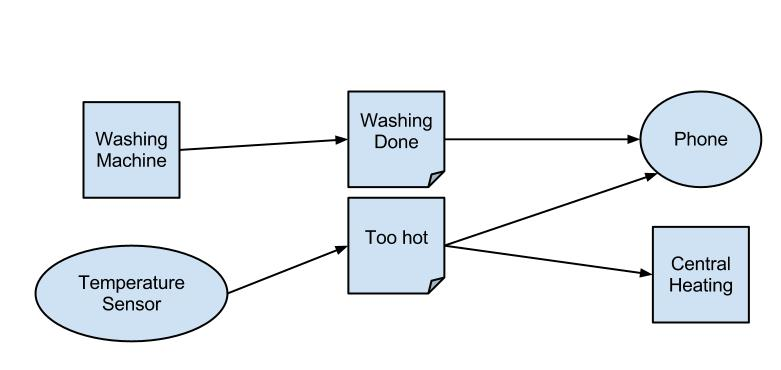
\includegraphics[scale=0.4]{images/JMS-IoT.jpg}
		\captionof{figure}{JMS Publish - Subscribe modelling IoT}\label{fig:JMS}
\end{figure}


Whilst JMS provides a well fitted framework, it does however come at a cost due to the runtime environment of Java and the additional overhead of having to run a separate server to glue the publishers and subscribers together. Whilst currently running the Java runtime on these constrained devices may not be possible, with the current pace of innovation, especially in optimisation of the Java runtime, and Moore's Law giving devices more power for the same cost and form factor every 18 months, it won't be long before it's really possible to have it running on the constrained devices of tomorrow. But until then, other alternatives and perhaps more suited tools, libraries and frameworks should be engineered starting at the lowest common denominator rather than shoe-horning large scale systems to fit constrained devices.


\begin{comment}
A fully featured pub sub system as well as point to point
pubs and subs don't know about each other but interact through Topics
Topics emulate the concept of a service very well i.e. Topic = bedroom light, living room thermostat. where subscribers can subscribe to events published to their topic

Great for large, high power machines.
Not so great on small, low power devices
JVM can be scaled down to lower power devices but still poses overhead to system.
\end{comment}
% subsection java_jms (end)

\newpage


\subsection{xAP} % (fold)
\label{sub:xap}

In the early 2000's, as an attempt to bring together a variety of technologies developed and used for Home Automation, an open source group decided to create a protocol to bridge the differences and create a unifying platform.\cite{xAP}

xAP, eXtensible Automation Protocol is designed to be a minimalist, elegant and easy to implement protocol with very basic requirements for the hardware, operating system, network and language on which it can run.  
The primary implementation is based on UDP/IP with a distributed architecture where no central controller co-ordinates the network. Instead, each device either transmits or listens for data on a broadcast channel. Their core justification for this is that the network becomes fault tolerant and can withstand devices disappearing off the network for one reason or another without having a detrimental effect on the whole network.

In this design there are two key classes of devices, senders and receivers, of which a device can be either or both. 
The receiver simply attaches to the network and listens for any incoming packets, it then chooses which ones are relevant to it and processes them.
The sender attaches to the network and broadcasts packets with payloads containing data relating to its service i.e. sensor data, incoming caller ID, etc. These packets only contain enough information to uniquely identify the source and the payload it wishes to send. There is no constraint on whether or not the packet must have a destination.

This design feature makes it very simple for new devices to attach to the network and start interacting without having to go through the process of setting up connections to other devices. It also makes it very easy to implement certain types of devices like loggers or informational displays which can collect data from all senders with relative ease. However, this also creates a huge strain on the devices attached to the network which all have to receive and process any broadcasted data, especially for those devices with limited resources. This becomes an increasing problem as more and more connected devices invade the home, from which the network will very quickly deteriorate as the volume of traffic being broadcast increases.

The protocol also defines a set schema for how packets should be formatted so that all devices can interoperate correctly. The schema covers both the header and the payload format, which is almost entirely text-based, resembling, albeit pre-dating, JSON, with the main intention of being human readable. Whilst so, this does come at the cost of not only increasing the size of the packet considerably with redundant text, but also the complexity in parsing the data with its varying delimiters. 

After the protocol's initial inception it has had limited success, even whilst it has been continuously developed over the years, it has done so in the shadows and not in an explicitly open and collaborative way, with no central repository for code collaboration/review and no single developer's forum for discussion. % POST LINK TO YAHOO FORUMS ETC

\begin{comment}
Core Idea is to build a distributed fault tolerant IoT protocol.
total broadcasting protocol, every device just beams out its own services and any device on the network can read and interpret the data.
Can be very inefficient for devices on battery(constant barrage) and doesn't scale well with 10's, 100's, 1000's of devices.
Designed to be hardware and link agnostic and to co-exist with other protocols. Basic implementation over UDP without any care for reliability AT ALL.

Purpose is that devices can hop on and off the network without breaking/severing the entire network.

Nice concepts and goals
BUT fails to deliver a system which can scale and do things efficiently
\end{comment}
% subsection xap (end)




\subsection{Remote Procedure Call - RPC} % (fold)
\label{sub:rpc}

% subsection rpc (end)
% section existing_systems_protocols (end)

\section{Developing systems} % (fold)
\label{sec:developing_systems}

\subsection{OpenWSN} % (fold)
\label{sub:owsn_berkeley}
Currently being developed at the University of California, Berkeley, the Open Wireless Sensor Network project is collection of open-source implementations of protocol stacks designed against to-be-finalised ``Internet of Things'' standards, for a range of different software and hardware platforms.

%TO BE CONTINUED


\subsubsection{CoAP} % (fold)
\label{ssub:coap}

% subsubsection coap (end)
% subsection owsn_berkeley (end)

\subsection{SmartThings} % (fold)
\label{sub:smart_things}
Launched in 2012, the SmartThings platform aims to allow the user to turn any ordinary object in the home into a ``Smart'' object by giving it the ability to connect to the Internet. The platform consists of a central hub connected to the Internet, containing a low-power Zigbee radio, from which it connects to an array of SmartThings accessories as well as many pre-existing third party Zigbee devices. Some of these accessories include motion detectors, moisture sensors, vibration detectors, power-plug switches as well as many others. The user can then connect to the SmartThings service through an Internet-connected pc or a smartphone, allowing them to either control the devices directly or set-up rules/schedules for devices, similar to the previously mentioned Twine device(\ref{sub:past_present_and_future}). 

Whilst providing easy to set-up pre-made SmartThings, the developer also provides the open-source Arduino kits to let hobbyists create their own SmartThings utilising the already well supported Arduino platform.

Currently, there is no information on how the underlying protocol for connecting the SmartThings to the hub works, but at the time of writing, the current implementation uses a ``cloud first'' approach. This means that rather than hub wiring all devices together based on the rules and schedules set up by the user, all the intelligence of the network is being handled in the cloud. This brings about the problem of Internet connectivity, with two points of failure, either the user or the cloud. From the user's standpoint, an Internet connection might not be available where the hub is located, or the user could have a faulty, slow or non-permanent connection, which renders all the SmartThings devices into dumb devices. In contrast to this, because of the reliance on the cloud, if the cloud service provider experiences downtime then all SmartThings users devices become dumb devices. In cases where these devices are used for security and safety, dire consequences could result.
  


% subsection smart_things (end)

\subsection{Qualcomm} % (fold)
\label{sub:qualcomm}
2013 CES Discussed bringing mobile platform hardware to IOT, but still creating a single device with internet as hub mainly 
% subsection qualcomm (end)
% section developing_systems (end)



% chapter background (end)
%==============================================================================


%==============================================================================

\chapter{Requirements gathering} % (fold)
\label{cha:requirments_gathering}
% Requirements of the hardware independent design
 
% Looking at xAP, JMS, what's wrong, how can that be resolved
% what are typical use cases/ types of devices

As discussed in the previous chapter, many different platforms and protocols exist to create an ``Internet of Things'' and most take very different approaches. This chapter will highlight several drawbacks of some the previously mentioned systems, explain how such problems can be resolved with this new approach and discuss the requirements for developing a new system, which is better suited for constrained devices and the environment of the ``Internet of Things''.

\section{Primary Requirements}
\label{sec:primary_requirements}
Due to the nature of the target hardware platforms, constrained devices such as Arduino and TelosB, heavyweight approaches become infeasible i.e., Java \& JMS. Therefore an extremely lightweight and scalable protocol, both in terms of the protocol data unit (pdu) and the complexity in processing and managing the runtime, is a primary requirement.

Secondary to this, because of the often unstructured and ad-hoc design of a typical ``Internet of Things'' network, building a centralised system i.e., a name server for device search, is an unnatural fit with the network. A single failure in the server could bring the entire network down, whilst all other devices are fully operational and no way to communicate with each other.
Instead, creating a distributed system which gives all the devices in the network the power to discover and communicate with each other, relieves the network of a single point of failure and can help spread the load. % ADD SOMETHING TO DO WITH DISCOVERY

Taking into consideration the typical types of devices connected to the ``Internet of Things'', three general roles of devices can be discerned; a sensor, an actuator and a controller. Sensors, anything from a temperature sensor to an open door sensor, provide a continuous service to other devices in the form of real-time data, usually from the outside world. Similarly, actuators also provide a service to other devices in the form of an interaction with the outside world, such as a speaker, light switch or thermostat. Lastly, controllers are devices which orchestrate the ``Things'' in the network, forming relationships between devices and creating useful interactions between the digital and real world i.e., connecting to both a door sensor and a light switch, when the door opens the light turns on. Whilst there are these distinct roles, it is often the case that one device could take on more than more role i.e., a light switch can both sense its state, and provide an action, turn on or off.


\section{Typical Use Cases} % (fold)
\label{sec:typical_use_cases}
This section will demonstrate several typical use case scenarios of different combinations of devices that an ``Internet of Things'' around the home may be composed of, with some necessary requirements in order to operate correctly.

\begin{itemize}
	\item Logging % single devices, no complex relationship
	\begin{itemize}
		\item The logging application runs on a controller device interacting with one or more sensors. The controller requests data from a temperature sensor and logs it to a file locally. The purpose of such an application can be to help with understanding the state of an area, room or home over a larger period of time, from which some assessment can be made e.g., one room is always warmer than the other during the afternoon. 
	\end{itemize}
	\item Presence detection lighting % Multiple devices, complex relationship
	\begin{itemize}
		\item The presence detection application runs on a controller device interacting with both a sensor and actuator devices. Within certain areas of the environment motion detectors are placed to detect the presence of a person in a particular space. This data is then communicated back to the controller and used to determine which lights to command to turn on or off. The purpose of this application would be to reduce the energy costs associated with lights unnecessarily left on.
	\end{itemize}
	\item Wash cycle complete
	\begin{itemize}
		\item The wash cycle complete application runs on a controller interacting with a sensor and an actuator. The actuator could be any form of communication medium that can alert the user i.e., sending a text message or tweet. This application would enable a washing machine to act as a sensor, relaying information back to the user(time left) and when a wash cycle has completed or requires further attention the user could be alerted in some form so that they can attend to it.
	\end{itemize}
	\item Direct control and observation
	\begin{itemize}
		\item A direct control application would allow a user to interact with the ``Internet of Things'' directly through a web browser or smartphone application. Such an application would operate on a controller device and allow a user to dynamically create new rules and relationships between existing devices as well as directly command devices such as lights, thermostats etc.
		This would allow a user to easily create and destroy relationships between devices without reconfiguring or restarting the network of devices.
	\end{itemize}
	\item Multi-decision heating
	\begin{itemize}
		\item A multi-decision application, such as a heating system, would take advantage of an arrangement of multiple different types of sensors and existing services. These sensors could include: temperature sensors to sense the current temperature of different spaces, presence sensors to detect where a person in the environment, location sensors to detect if someone is actually home. The combination of these sensors could allow the system to detect whether the environment should be heated, and if so when and by how much. Building upon the initial use case of logging, a logger could be used to create a basic schedule of when people are in the environment so that heating schedules can be created, this would allow the environment to be heated upon the arrival of someone.
	\end{itemize}
\end{itemize}

% subsection typical_use_cases (end)

\section{Functional Requirements} % (fold)
\label{sec:functional_requirements}
This section describes the functional requirements which were gathered and are based upon the needs of the use cases discussed in the previous section.
% section functional_requirements (end)
\begin{enumerate}
	\item Support 3 device roles; Sensor, Actuator, Controller
	\begin{itemize}
		\item These 3 roles of devices are needed to form the basic closed loop interaction model necessary for the ``Internet of Things''.
	\end{itemize}
	\item Configuration of device attributes both at compile time and run time i.e., name, type, frequency, etc.
	\begin{itemize}
		\item This is necessary in order make each device distinct from another, as well as customise it based on its needs, either in terms of performance, power constraints or otherwise. By enabling run time configuration it simplifies updating the devices on the network without the need to recompile.
	\end{itemize}
	\item Discovery/querying of devices
	\begin{itemize}
		\item Discovery of other devices on the network is a core feature of a distributed ``Internet of Things'' network, without this the network can't dynamically grow by finding new devices. Querying of devices is to determine compatibility of devices before making a connection, by filtering out requests which don't match a devices attributes network congestion can be reduced.
	\end{itemize}
	\item Negotiation and connection to devices
	\begin{itemize}
		\item Negotiation is necessary to determine the characteristics of the relationship between two devices, which is based on the demands of the device initiating the connection and whether or not the recipient can or wants to meet that demand i.e., a device can request a certain frequency of readings from another device which may or may not be able to match it.
	\end{itemize}
	\item Closing connections to devices
	\begin{itemize}
		\item Devices need to be able to gracefully close any formed connections, which could be due to limited power constraints or no longer needing the resources that the connection offers. These connections also must be closed gracefully, in contrast to just not responding/dissappearing off the network, in order to ensure that a device's resources are not wasted by keeping state for a terminated connection, which could be confused for transient communication loss.
	\end{itemize}
	\item Sensors must be able to send data to controllers
	\begin{itemize}
		\item A sensor's core functionality is collecting data through sensing the environment, this data may be of interest to other devices on the network and therefore must able to to send it to them. These data transmissions also need to be sent at a set frequency, either configured or negotiated, so that a receiving device knows when to expect data.
	\end{itemize}
	\item Actuators must be able to receive commands from controllers
	\begin{itemize}
		\item An actuator's core functionality is interacting with the environment, without informed control of the device it has no use by itself. Therefore the device must be able to accept commands from other devices, such as controllers, in order to interact with the environment with a purpose.
	\end{itemize}
	\item Controllers must be able to send commands to actuators and receive data from sensors
	\begin{itemize}
		\item A controller's purpose in the network is to form connections to other devices to create the closed loop system, which in order to do this, must be able to receive data from sensors and send commands to actuators. 
	\end{itemize}
	\item All device roles must support connections to multiple devices 
	\begin{itemize}
		\item This is necessary in order to allow a device to form relationships to several other devices, which not makes better use of the available resources within each device but also allows for devices to form multiple, more complex relationships between different devices i.e., a temperature sensor connecting to one controller which logs its data and to another controller which is connected to an actuator that controls the thermostat.
	\end{itemize}
	\item Liveness checks through pings
	\begin{itemize}
		\item Due to the distributed and unreliable nature of the network environment, devices need to be able to check the liveness of the connections to ensure devices are still active, and for those that aren't, react gracefully by cleaning up the expired connection and perhaps try to discover new devices.
	\end{itemize}
	\item Application Protocol Interface
	\begin{itemize}
		\item This is necessary for applications to be built on top of the device roles, which will utilise the capabilities of the underlying network of ``Things'' to create rich and powerful systems in the ``Internet of Things''.
	\end{itemize}
\end{enumerate}

\section{Non-Functional Requirements} % (fold)
\label{sec:non_functional_requirements}
This section describes the non-functional requirements based on the expectations of the system, its performance characteristics and the requirements for developing the project as a whole.
\subsection{System Requirements} % (fold)
\label{sub:system_requirements}
\begin{itemize}
	\item Closed loop system
	\begin{itemize}
		\item The system must be able to sense, process and react within the network itself, to create a fully reactive closed loop system.
	\end{itemize}
	\item Lightweight
	\begin{itemize}
		\item Because of the target systems, constrained devices, the system must be lightweight enough, both in terms of the protocol data unit and use of system resources, so that devices such as the TelosB mote can run it.
	\end{itemize}
	\item Scalable, from small to large networks of devices
	\begin{itemize}
		\item Because of the rapid adoption of technology within our environment, the system must be able to scale from small to large networks in order to support the use of 10's if not 100's of devices with a single network, without causing unnecessary congestion and still ensuring the same performance of smaller networks.
	\end{itemize}
	\item Cross platform compatibility
	\begin{itemize}
		\item Due to the heterogeneous nature of hardware and software platforms available today, the system must be designed in such a way so that it is both hardware and software independent, enabling it to be implemented on these platforms as well as across a variety of networks.
	\end{itemize}
	\item Simple to extend
	\begin{itemize}
		\item Due to the constantly evolving nature of technology the system must be extensible in order to support new types of devices, and also be able to support new payloads specific to these devices.
	\end{itemize}
	\item Reliability of essential communications
	\begin{itemize}
		\item Because of the reliability concerns regarding the underlying network, building in some reliability is necessary to ensure that critical communications are successful, such as forming connections between devices. 
	\end{itemize}
	\item Basic assurance of correct data
	\begin{itemize}
			\item Due to the reliance upon data within the network in order to sense, process and react to the environment, all data transferred must be reliable, therefore the need for some checks to ensure it is correct when it reaches the destination are needed. 
	\end{itemize}
	\item Network resilience to device failures
	\begin{itemize}
		\item Because of the unpredictable nature of the environment and the limited capabilities of some devices (battery powered), the system must react gracefully to device failures, without the entire system being rendered in-operational.
	\end{itemize}
	\item Liveness monitoring
	\begin{itemize}
		\item The system must be able to monitor and react to the liveness of devices in the network i.e., if a device becomes unreachable, close connection gracefully and clean up.
	\end{itemize}
	\item System performance
	\begin{itemize}
		\item Because of the real-time nature of the ``Internet of Things'', the system must perform suitably, so that data is received and commands are carried out within acceptable real-time bounds i.e., receiving temperature readings for an hour ago are of no use to a device which shows the user the current temperature.
	\end{itemize}
	\item Device resources
	\begin{itemize}
		\item The system must consume as little device resources as possible in order to support the development of user applications on top.
	\end{itemize}
\end{itemize}
%How the system should perform
%LIGHTWEIGHT, SCALABLE
%Resilience, discovery, reliability, pinging

% subsection system_requirements (end)

\subsection{Development Constraints} % (fold)
\label{sub:development_requirements}
\begin{itemize}
	\item The system must be researched, designed and developed within a limited time frame, about 20 weeks.
	\item The choice of platforms for implementing the design is based on the availability of constrained devices between the School of Computing Science and the author.
	\item The choice of operating system for the constrained device is based on prior experience with similar systems and platform languages available to the OS. The Contiki OS uses a minor variation of the C programming language, making it quicker and simpler to get started based on the author's experience with C, as well as simpler to keep the system (mostly) platform independent.
\end{itemize}
% subsection development_requirements (end)
\subsection{Development Assumption} % (fold)
\label{sub:development_assumption}
In order to design and implement the proposed system, the scope of the problem needs to the limited, therefore it becomes necessary to define several assumptions.
\begin{itemize}
	\item The number of possible devices types is limited, no more than 255.
	\item Sensor data is not critically important, so packet loss is acceptable.
	\item The system will be used in an environment where security is a non-issue (but MUST be considered as future work before deployment).
\end{itemize}
% subsection development_assumption (end)

% section non_functional_requirements (end)




%Heavy weight Java
%Centralised
% selective reliability, ephemeral data
%XAP wasteful, doesn't scale
%not easy to parse
%Some request response
%Simple to implement, simple to extend, MULTICAST, UNICAST, 
%Joining devices together rather than lone wolves connecting, cheapening links




% chapter requirments_gathering (end)
%==============================================================================


%==============================================================================


\chapter{Design} % (fold)
\label{cha:design}
% SETTINGS
\definecolor{lightgray}{gray}{0.8}
\newlength{\maxheight}
\setlength{\maxheight}{\heightof{W}}

\newcommand{\baselinealign}[1]{%
	\centering
	\raisebox{0pt}[\maxheight][0pt]{#1}%
}
%END OF SETTINGS


% Design of system independent of hardware implementation.
This chapter describes and illustrates the design of the new protocol, independent of any hardware and software platforms, as set out by the requirements gathered in the previous chapter. This chapter will discuss the different roles of devices to be used, the fundamental features necessary to meet the requirements, the types and flow of messages between the different roles, the protocol data unit and command formats defined and finally some of the key design choices for this protocol will be compared to decisions made by other pre-existing protocols, to highlight and discuss their differences and/or similarities.

\section{The three device roles} % (fold)
\label{sec:the_3_classifications_of_devices}
In order to understand and design the system correctly, the three basic device roles in the ``Internet of Things'' must be explicitly defined; these roles will ultimately dictate the core communication model between devices in the network. However, whilst these roles are distinct in nature, a single device may take on one or more roles, e.g., a light sensing its state, and offering a command to turn it on/off.

By separating out functionality into distinct roles, it enables each to device to offer individual, context-less services which can be offered to many different devices and combined to create a powerful, rich and adaptable ``Internet of Things''.

\subsection{Sensor} % (fold)
\label{sub:sensor}
The sensor is \textit{the} key component of any ``Internet of Things'' network; without the ability to sense, either on demand, periodically or in real time, the user is forced to consciously interact with the system, in turn defeating the purpose of the ``Internet of Things''.

The sensor in the ``Internet of Things''can be seen as a simple device which does little to no computation, except that of formatting or preprocessing the data it senses, and simply forwards it to one or more devices in the network that have expressed interest in its data, at set time intervals. These intervals can be decided either by the sensor or the interested device, based upon the needs and resources available to both.

Because data from sensors is usually of an ephemeral nature, recovery/retransmission of damaged/lost packets is usually not of interest after the next one in the sequence has arrived, e.g., no need for previous temperature readings when interested in the current temperature now. However, knowing that the data has arrived correctly and undamaged is of importance, as data must be correct for the system to operate correctly and as expected.
% subsection sensor (end)

\subsection{Actuator} % (fold)
\label{sub:actuator}
Actuators, like sensors, are a key component in the ``Internet of things'', performing actions to interact with the real world, e.g., turn on light or display the current temperature. Without the use of actuators, the system would only be able to record and process the environment without having anyway of reacting to any events.

By themselves actuators are primitive devices and are only able to perform context-less actions by themselves, e.g., turn on and off a light. In order to create meaningful actions, such as turning on a light when someone enters the room, actuators need to be able to offer their actions, or functions, as a service to other devices in the network whom are interested in performing such actions.

Because of the on-demand semantics of performing an action, actuators need to be always available and ready to respond to incoming commands at any time. In order to ensure that these commands are carried out successfully and not lost in transit, a reliable connection will need to be formed between the controller and actuator.
% subsection actuator (end)

\subsection{Controller} % (fold)
\label{sub:controller}
Controllers, unlike sensors and actuators, are the brains of the ``Internet of Things''; by themselves, they can do nothing, but by utilising other devices in tandem, they can create a powerful, sensing and reactive system. 

By connecting to sensors, controllers can give the data sensed a purpose and meaning, and by connecting to actuators it can give actions a reason to be performed, e.g., when the temperature sensor readings are \textgreater 26C, the room is too warm, therefore turn down the thermostat, in order to reduce the temperature to a more preferable setting. 

Within a single network it is possible to have several controllers all connected to the same or different devices as well as connected to each other, and each could perform different functions in the network i.e., one controller logs all devices in the network, one controller controls living room devices and another controls bedroom devices. Extending this, allowing controllers to connect to one another enables the network to form more complex relationships to perform actions that one controller alone could not, such as one controller having Internet connectivity providing resources such as cloud connectivity to the other controllers.
% subsection controller (end)
% section the_3_classifications_of_devices (end)


\section{Protocol Design} % (fold)
\label{sec:protocol_design}
This section discusses the design of the protocol based on the formal requirements, from the basic sequence of messages passed between the different roles, to deriving specific state machines for each role.

\subsection{Features} % (fold)
\label{sub:features}
The protocol is designed to fulfil several key requirements:\vspace{-5mm} 
\begin{itemize}
	\item Minimalistic protocol, reliability for critical data only, no fragmenting
	\item Minimal header overhead, reduce transmission and receiving cost of data
	\item Distributed device discovery, use of broadcast to discover devices
	\item Reliability, reliable set-up of connections and integrity of data
	\item Fault tolerant, liveness checks and no central point of failure
\end{itemize}
% subsection features (end)


\subsection{Transport Layer}
Due to the requirements of the protocol, allowing it to run on a variety of networks, and reducing necessary transmissions to save power, the design of the protocol is such that it only requires packets to be sent over a best effort link with no reliability guarantees; instead the protocol itself handles any problems with corrupt data or dropped packets, as discussed later in this section,\ref{sub:selective_reliability}, \ref{sub:data_integrity}. 

The one significant requirement of the transport layer is that it must provide the capability to send both broadcast and unicast packets, due to the device discovery requirement.
Therefore, a simple datagram transport layer can be used to provide the required functionality, such as the IPv4/6 User Datagram Protocol (UDP) or Contiki Rime stack\cite{RimeStack}.

\subsection{Multiplexing devices, channels}
In order to enable devices to communicate with more than one other device, a method for multiplexing a device's resources must be created. Within this system, each connection between two devices is called a channel, and each device can serve multiple channels, depending on its own resources, i.e., the more resources available, the more channels a device can serve, the more devices a single device can connect to. 

Each device will contain at least two channels, one home channel (default) and one or more ephemeral channels. The purpose of the home channel is to enable devices to have a well known location at which they can be contacted; this will be used for device discovery and to request to start a connection on one of the ephemeral channels.

In order to uniquely identify each connection, a triple of identifiers is required:\vspace{-5mm} 
\begin{itemize}
	\item transport layer address of each host the system is running on (IP address or Rime address).
	\item transport layer multiplexing identifier associated with the running system process (UDP port or Rime channel).
	\item a multiplexing identifier for each connection to a device, called a channel.
\end{itemize}

\subsection{Selective Multicast/Unicast} % (fold)
\label{sub:selective_multicast_unicast}
The use of multicast in a network can be extremely expensive, both in terms of the bandwidth consumed on the network as well as the time and energy cost of every device being forced to receive and process the packet. Therefore multicast transmissions must be kept to a minimum and where they are necessary, ensure that it is not used excessively.

In the case of device discovery, multicasting is required due to the distributed nature of the system, where no central name server exists and therefore the network needs to be queried in order to locate devices. In order for this to work, all devices on the network need to listen on a well known address (e.g. UDP port), to which the discoverer can send multicast discovery packets.
Once a device receives a multicast discovery packet, it can decide whether or not to reply, based on whether the query information, device type or name, matches its own. If it does match, then it replies using a unicast message to notify the sender of an available device matching its request. Because filtering is used at the receiving end, this further reduces the strain on the network resources, by stopping unnecessary packets from being transmitted.   
% subsection selective_multicast_unicast (end)

\subsection{Selective Reliability} % (fold)
\label{sub:selective_reliability}
In an effort to both reduce the cost of data transmission for devices and bandwidth consumption on the network, reliability will only be ensured for critical data transmissions, including connection set-up, tear-down and actuator commands.

Because of the unreliable nature of the underlying network, ensuring that connections are formed correctly is extremely important, otherwise a connection forming packet might be dropped, causing one device to believe the connection has been fully set-up whilst the other waits for the dropped packet which will never arrive. 
Another case where this is important is when issuing commands to actuators, as it is necessary to ensure actions are in fact carried out and the command hasn't been lost on the network. This can achieved through at-least-once semantics, ensuring that the actuator receives at least one command, so that it performs the action, and any repeat requests can be ignored.

Whereas, when sending data such as sensor readings the reliability of it arriving is not as important, this is largely attributed to the ephemeral nature of sensor readings, especially in a real-time environment like the ``Internet of Things''. For example, in a scenario where the current temperature is being displayed to the user, the need for old, out of sequence data, which may have been lost and retransmitted becomes unnecessary, as the user is only interested in the current temperature.
% subsection selective_reliability (end)


\subsection{Liveness response} % (fold)
\label{sub:liveness_response}
In order to ensure the connections between devices are kept alive, the liveness of a connection needs to be tracked, this is done differently depending on the device.
\begin{itemize}
	\item [Sensor -] Because sensors transmit data back to a controller at a set frequency, the controller can easily keep track of the liveness by simply monitoring incoming packets. If an arbitrary number of packets is not received after a multiple of the frequency period, then a time-out will occur and the connection can then be probed using a PING message to check if the packet loss is transient. If no responses are received in the form of PACKs, then the connection can be closed gracefully. 
	\item [Actuator -] Because actuators just listen on the connection for any commands from a controller, it becomes necessary to regularly check at an arbitrary frequency that the connection is still alive using PINGs. Without PINGs, if a command was sent, it would initially be difficult to tell whether the packet was lost or the connection is dead. By using PINGs, the status of the connection to the actuator can be regularly monitored, and if necessary, the associated channel closed when the actuator is persistently unresponsive.
	\item [Controller -] Because controllers actively keep track of actuators, actuators therefore implicitly know that the controller is still alive. However, this is not the case for sensors, which are only liveness checked passively unless there is packet loss. Because of this, the sensor must therefore regularly send PINGs at an arbitrary frequency to check to see if the controller is still alive to receive the packets of data being transmitted. If this was not checked, then the sensor would be not only wasting its own resources by needlessly sending data, but it would also consume the resources of other devices if this was deployed on a low-power multi-hop mesh network, typical for ``Internet of Things'' networks.
\end{itemize}

In order to ensure the network does not become congested by the retransmission of PINGs within a short period of time, an exponential back-off will be used. This will ensure that if a device were to disappear off the network, the rest of the network would not suffer. In a large network where multiple devices could fail at once, perhaps due to a common link, the network could become heavily congested if exponential back-off were not used.

If after an arbitrary number of PINGs, a PING ACK is not received, the connection is deemed dead and the associated channel closed.
% subsection liveness_response (end)

\subsection{Data integrity}
\label{sub:data_integrity}
Whilst most data sent in the ``Internet of Things'' network does not need to be sent reliably, due to it's ephemeral nature, it is important however that when it arrives it is consistent and accurate; if sensor readings were to become corrupt in transit, then unintended actions could result from inaccurate data. For example, a temperature sensor transmits the current temperature to a controller, which becomes corrupt in transit, as a result of the corrupt sensor reading, the controller believes the current temperature is too hot and the thermostat is commanded to turn off, when in fact the temperature was at an acceptable level.

Therefore, the use of a mechanism to ensure the integrity of the data is necessary, such as a Cyclic Redundancy Check, CRC. In this protocol, a 16bit CRC will be used to ensure that when data is sent from one device to another, that it is possible to discern whether or not it is accurate and consistent. If the integrity of the data is found to be compromised, then the packet will simply be dropped. If the packet was sent as reliable data (connection request or command), a timeout will occur in the sender device expecting an acknowledgement, and the packet will be resent. 



\subsection{Flow of messages} % (fold)
\label{sub:message_passing}
Based upon the use cases described in the Requirements section, a set of messages are described and demonstrated in the sequence diagram contained in figure \ref{fig:sequence_diagram}, which illustrates the flow of messages between the different roles of devices within the network.

\subsubsection{Device discovery -- Controller $\rightarrow$ Sensors/Acutators} % (fold)
\label{ssub:subsubsection_name}
In order for a controller to locate devices on the network, a device query must be broadcast across the network; any devices which match the request and have resources available can reply with an acknowledgement, otherwise they ignore the message, implicitly signalling no.
If a controller receives no responses from the initial query, it could be a result of either, no devices on the network matching the request, or a response packet was lost/corrupted on the network. Because it's not possible to distinguish between an implicit no and a network failure, it may be necessary to retransmit a query multiple times, perhaps with an exponential back-off, so as not to congest the network whilst still achieving a confident scan of the available devices on the network.

% subsubsection subsubsection_name (end)

\subsubsection{Set up channel -- Controller $\rightarrow$ Sensors/Actuators} % (fold)
\label{ssub:set_up_channel}
In order to ensure that a channel is fully set up, it becomes necessary to introduce reliability, via acknowledgement messages. Similar to TCP, a three-way handshake is used to ensure the channel is fully opened on both sides.
\vspace{-5mm} 
\begin{itemize}
 	\item This covers most scenarios and allows for devices to recover from dropped packets during the exchange. For example, device A initiates setting up a channel,
 	\begin{itemize}
 		\item if the initial message is dropped, an acknowledgement timeout occurs on A, A then resends message.
 		\item if B's ACK is dropped, an acknowledgement timeout occurs on A, A then resends the message with the same sequence number, when B receives the initial message again, its ACK message must have been dropped, so B resends the ACK message.
 		\item if A's ACK message is dropped, an acknowledgement timeout occurs on B, then B resends the second message with the same sequence number, when A receives B's ACK message again, its ACK message must have been dropped, A then resends the ACK message.
 		\item if A receives no more ACK messages from B, it knows the channel has been fully set up.
 	\end{itemize}
 \end{itemize} 
% subsubsection set_up_channel (end)

\subsubsection{Send sensor data -- Sensor $\rightarrow$ Controller} % (fold)
\label{ssub:send_sensor_data}
Once a channel has been set up to a controller, a sensor then needs to send its sensor readings at the previously agreed upon frequency. 
Due to the high frequency requirements and transient nature of the data, using reliability becomes an expensive overhead without providing much benefit, i.e., consuming twice the bandwidth, and if a packet is dropped and resent out of sequence it becomes useless in a real-time environment, like the ``Internet of Things''.  
Without reliability, packets may be dropped, but because of the timeliness of the data it will usually go unnoticed to the user. For example, a dropped packet won't have noticeable effect on a real-time temperature display with a frequency granularity of 5 seconds.
% subsubsection send_sensor_data (end)

\subsubsection{Send command -- Controller $\rightarrow$ Actuator} % (fold)
\label{ssub:send_command}
Once a channel has been set up to an actuator, a controller needs to be able to send it commands to carry out. To ensure that an action is carried out, it becomes necessary to acknowledge each command. By using acknowledgements in combination with message sequence numbers, it is possible to ensure that a command is carried out exactly once per request.
\vspace{-5mm} 
\begin{itemize}
	\item The following cases are covered via the use of acknowledgements and sequence numbers
	\begin{itemize}
		\item if command message is dropped, an acknowledgement timeout occurs on the controller, controller then resends command.
		\item if ACK message is dropped, an acknowledgement timeout occurs on the controller, controller then resends command with the same sequence number, when the actuator receives repeat commmand, it ignores command and resends ACK message.
	\end{itemize}
\end{itemize}

% subsubsection send_command (end)

\subsubsection{Ping -- All roles} % (fold)
\label{ssub:ping}
Once a channel has been set up between two devices, it is possible for one to disappear without closing the channel gracefully, which could be due to various reasons e.g., loss of battery power, failed network link, device failure, etc. Therefore it becomes necessary to test the channel and see if the other participant is still alive, terminating it and cleaning up the channel if not.

Other cases for its use in this protocol are the following: for the controller to check that the channel to the actuator is still alive, and for the sensor to check that the controller is still alive to receive its data, ensuring network resources are not being wasted sending data to a disconnected controller.

To test the channel a PING is sent from one device to the other, with the expectation of receiving a PING ACK to signify the channel is alive.
% subsubsection ping (end)

\subsubsection{Close channel -- All roles} % (fold)
\label{ssub:close_channel}
Once a channel has been set up between two devices, one of the devices may decide at a later time that it either no longer needs the services provided by the channel, or is unable to support it, perhaps due to limited power. Therefore, it becomes necessary to close the channel gracefully, ensuring the both ends understand the channel is closed and all associated state destroyed. In order to ensure the channel is closed on both sides correctly, an acknowledgement must be used to signify the other side received the command.
\vspace{-5mm} 
\begin{itemize}
	\item The following cases are covered via the use of acknowledgements between devices A and B:
	\begin{itemize}
		\item if the close channel message sent from A is dropped, an acknowledgement timeout occurs on A, A then resends the message.
		\item if B's ACK message is dropped, an acknowledgement timeout occurs on A, A resends the close channel message, when B receives the message it checks for any channel associated to A and closes it (if not done already), then resends the ACK message to A.
	\end{itemize}
\end{itemize}


% subsubsection close_channel (end)
\begin{figure}[h!]
\centering
\includegraphics[scale=0.5]{design/img/sequence_diagram.1}
\caption{Controller - Sensor message diagram}
\label{fig:sequence_diagram}
\end{figure}
% subsection message_passing (end)



\newpage
\subsection{Protocol state machines} % (fold)
\label{sub:states}
With the use of the message sequence diagrams to help understand the flow of messages within the network, the sequence of states each connection within a role can transition between can be discerned, and is shown in the following figures.

Within these diagrams, a number of message types are show as labels on the transitions between the various states within each system, these message types are later described in the next section, \ref{sec:protocol_data_unit}

\subsubsection{Sensor} % (fold)
\label{ssub:sensor}
\begin{figure}[h!]
\centering
\includegraphics[scale=0.65]{design/img/sensor_state.1}
\caption{Sensor life cycle diagram}
\label{fig:sensorstate}
\end{figure}


% subsubsection sensor (end)
\subsubsection{Actuator} % (fold)
\label{ssub:actuator}
\begin{figure}[h!]
\centering
\includegraphics[scale=0.65]{design/img/actuator_state.1}
\caption{Actuator life cycle diagram}
\label{fig:actuatorstate}
\end{figure}
% subsubsection actuator (end)

\subsubsection{Controller} % (fold)
\label{ssub:controller}
\begin{figure}[h!]
\centering
\includegraphics[scale=0.65]{design/img/controller_state.1}
\caption{Controller life cycle diagram}
\label{fig:controllerstate}
\end{figure}


% subsubsection controller (end)


% subsection states (end)




\section{Protocol Data Unit} % (fold)
\label{sec:protocol_data_unit}
This section discusses and illustrates the design of the Protocol Data Unit (PDU), starting with the protocol header format and followed by the various message types and their respective payload formats. Where appropriate, for each message type, a short pseudo code analysis will be discussed to illustrate the various scenarios that could occur in the relevant state machine, as a result of receiving the respective messages.

\subsection{Protocol Header} % (fold)
\label{sub:protocol_header}
The design of the protocol header tries to minimise the overall size by only containing a minimal set of non-textual data fields, with the purpose of reducing the power consumption for transmitting and receiving packets. The included fields are essential for identifying channels, distinguishing message types and ensuring the integrity of the data transmitted.

The protocol header contains 6 data fields:
\vspace{-5mm}  
\begin{itemize}
	\item source and destination channel fields to identify the connection (used with lower layer addressing to uniquely identify each connection),
	\item a sequence number field to detect duplicates and out of order packets,
	\item a command field to distinguish what type the payload is,
	\item a payload length field which contains the size of the payload, maximum size = 32 bytes
	\item and a checksum is computed over the entire packet to detect any errors that might have occurred during in transmission.
	\begin{itemize}
	 	\item When initially computed for the packet, the checksum field is filled with 0's and then filled with the result. Once received, the checksum can then be recomputed and the result should be 0 if the packet is correct.
	 \end{itemize} 
\end{itemize}    
% subsection protocol_header (end)
\begin{figure}[h!]
\begin{center}
\begin{bytefield}{32}
\bitheader{0,8,16,24,31}\\
	\begin{rightwordgroup}{Header}
		\bitbox{8}{Src channel} & \bitbox{8}{Dest channel} & \bitbox{8}{SeqNo} & \bitbox{8}{Command} \\
		\bitbox{16}{Payload length} & \bitbox{16}{Checksum}
	\end{rightwordgroup}\\
	\wordbox[lrt]{1}{Command specific payload}\\
	\skippedwords \\
	\wordbox[lrb]{1}{}
\end{bytefield}
\caption{Protocol header format}
\end{center}
\end{figure}

To further illustrate the different classes of messages and how they relate to the header, a packet class digram is shown in figure \ref{fig:packet}.

\begin{figure}[h]
\centering
\includegraphics[scale=0.5]{design/img/PacketHierachy.1}
\caption{Message hierarchy}
\label{fig:packet}
\end{figure}
% subsection protocol_data_unit (end)

\section{Payload Message Types and Formats} % (fold)
\label{sec:payload_formats}
This section discusses the various payload message types which can be sent, and the associated actions taken upon receiving a message.
For each message type the payload format is described and illustrated.
\subsection{QUERY} % (fold)
\label{sub:query}
Before a controller can connect to any devices, it must first try to discover any matching devices on the local network. To do this, the device's home channel sends a QUERY message to the home channel on every other device in the network.
\vspace{-5mm} 
\begin{itemize}
	\item []The receiving state machine does the following on receipt of a QUERY message:
	\begin{itemize}
		\item if the destined channel is the home channel, it checks the type field, 
		\begin{itemize}
			\item if it matches its own type then transmits a unicast QUERY Response message back to the sender.
			\item if the type does not match, message is dropped and device does not respond.
		\end{itemize}
		\item if the destined channel is not the home channel, the message is dropped as the requesting channel is confused.
	\end{itemize}
\end{itemize}

The QUERY message contains two data fields: the type of device the controller is searching for, light sensor, temperature sensor, informational display or otherwise, and the name of the device sending the QUERY message. This packet is sent as a broadcast transmission to all devices on the network.

\begin{figure}[h!]
\begin{center}
\begin{bytefield}{32}
\bitheader{0,8,16,24,31}\\
\bitbox{8}{type} & \bitbox[lrt]{24}{}\\
\wordbox[lrb]{1}{name = 16 bytes}
\end{bytefield}
\caption{QUERY message payload format}
\end{center}
\end{figure}
% subsection query (end)

\subsection{QUERY Response} % (fold)
\label{sub:query_response}
After a device receives a QUERY message, it can decide whether or not to reply to it, based on a type match and if there are resources available, if so it replies with the QUERY Response message. 
\vspace{-5mm} 
\begin{itemize}
	\item []The receiving state machine does the following on receipt of a QUERY Response message:
	\begin{itemize}
		\item if destined for the home channel, it accepts all messages and passes them up to any application on top.
		\item if not destined for the home channel, then the message is dropped as the requesting channel is confused.
	\end{itemize}
\end{itemize}		
		
The QUERY Response message contains 3 data fields: the type and name of the device which is responding and the rate, which either indicates the default rate that a sensor transmits readings at, or the rate at which an actuator will expect PING messages from a connected controller to confirm the connection is still alive.
\begin{figure}[h!]
\begin{center}
\begin{bytefield}{32}
\bitheader{0,8,16,24,31}\\
\bitbox{8}{type} & \bitbox{16}{rate} &\bitbox[lrt]{8}{}\\
\wordbox[lrb]{1}{name = 16 bytes}
\end{bytefield}
\caption{QUERY Response message payload format}
\end{center}
\end{figure}
% subsection query_response (end)

\subsection{CONNECT} % (fold)
\label{sub:connect}
Once a device has been located, either \textit{a priori} or through querying, a controller needs to send a CONNECT message to start the process of creating a channel with the desired device. As shown in the message sequence diagrams, this uses a three-way handshake, of which this is the initial message. 
\vspace{-5mm} 
\begin{itemize}
	\item []The receiving state machine does the following on receipt of a CONNECT message:
	\begin{itemize}
		\item if destined for the home channel, and the device has not previously allocated a channel for the requesting device, it checks if the rate is compatible with its own,
		\begin{itemize}
			\item if compatible, it creates a new channel for this connection, sets it to the CONNECT sent state and responds with an accepting CONNECT ACK from the new channel.
			\item if not, respond with a declining CONNECT ACK.
		\end{itemize}
		\item if it has already allocated a channel for the requesting device and is in the CONNECT sent state, then the CONNECT ACK must have been lost, CONNECT ACK is resent.
		\item if it has allocated a channel for the requesting channel and is in the CONNECTED state, then the requesting device state machine is confused.
		\item if not destined for the home channel, then the requesting channel state machine is confused.
	\end{itemize}
\end{itemize}	


The CONNECT message contains 2 data fields: the rate at which the controller wants to either receive data readings from sensors, or receive PINGs from actuators, and the name of the controller.

\begin{figure}[h!]
\begin{center}
\begin{bytefield}{32}
\bitheader{0,8,16,24,31}\\
\bitbox{16}{rate} & \bitbox[lrt]{16}{}\\
\wordbox[lrb]{1}{name =16 bytes}
\end{bytefield}
\caption{CONNECT message payload format}
\end{center}
\end{figure}
% subsection connect (end)

\subsection{CONNECT ACK} % (fold)
\label{sub:connect_ack}
Once a device receives a CONNECT or CONNECT ACK message, unlike when receiving a QUERY message, it must respond with the second or third part of the three-way handshake with either a positive or negative acknowledgement in order to ensure the connection has been set-up fully. When responding to a CONNECT or CONNECT ACK message, the device can either accept the connection or decline it, which could be based on device being unable to match the demands from the controller or due to a lack of available resources needed to support the connection.
\vspace{-5mm} 
\begin{itemize}
	\item []The receiving state machine does the following on receipt of a CONNECT ACK message:
	\begin{itemize}
		\item if destined for an ephemeral channel which is in the CONNECT sent state,
		\begin{itemize}
		 	\item check if the connection has been accepted, if so reply with another CONNECT ACK.
		 	\item otherwise, close the newly opened channel.
		\end{itemize} 
		\item if destined for an ephemeral channel which is in the CONNECT ACK sent state,
		\begin{itemize}
		  	\item check the accept field to confirm the connection has been fully accepted, if so move to the CONNECTED state
		  	\item otherwise, close the newly opened channel.
		\end{itemize} 
		\item if destined for an ephemeral channel which is in the CONNECTED state, third handshake (CONNECT ACK) must have been lost, resend CONNECT ACK.
		\item if destined for an ephemeral channel which has not been allocated or does not exist, requesting channel must be confused.
		\item if destined for home channel, requesting channel is confused.
	\end{itemize}
\end{itemize}
The CONNECT ACK message contains 2 data fields: accept, which declares whether or not the recipient accepts to create a channel, and the name of the device sending the message.

\begin{figure}[h!]
\begin{center}
\begin{bytefield}{32}
\bitheader{0,8,16,24,31}\\
\bitbox{8}{accept} & \bitbox[lrt]{24}{}\\
\wordbox[lrb]{1}{name = 16 bytes}
\end{bytefield}
\caption{CONNECT ACK message payload format}
\end{center}
\end{figure}
% subsubsection connect_ack (end)

\subsection{RESPONSE} % (fold)
\label{sub:response}
Once a channel has been set up and is in the connected state, the sensor connected to the channel can then send RESPONSE messages containing its sensor readings at the previously agreed upon rate.
\vspace{-5mm} 
\begin{itemize}
	\item []The receiving state machine does the following on receipt of a RESPONSE message:
	\begin{itemize}
		\item if destined for an ephemeral channel which is associated with the sender channel and in the CONNECTED state
		\begin{itemize}
			\item accept the data and pass to application on top
		\end{itemize}
		\item if destined for an ephemeral channel which is associated with the sender channel, but is not in the CONNECTED state, then sender is confused.
		\item if destined for an ephemeral channel which is not associated with the sender channel, then sender is confused.
		\item if destined for home channel, then sender is confused.
	\end{itemize}
\end{itemize}


The RESPONSE message contains 2 data fields: the data being sent, for example a temperature reading or a light reading, and the name of the sensor. 

\begin{figure}[h!]
\begin{center}
\begin{bytefield}{32}
\bitheader{0,8,16,24,31}\\
\bitbox{16}{data} & \bitbox[lrt]{16}{}\\
\wordbox[lrb]{1}{name = 16 bytes}
\end{bytefield}
\caption{RESPONSE message payload format}
\end{center}
\end{figure}
% subsection response (end)

\subsection{COMMAND} % (fold)
\label{sub:command}
Once a channel has been set up between a controller and actuator, the controller can then send COMMAND messages to the actuator indicating that it needs to perform its action. This is part of a reliable request-response sequence of messages and expects an acknowledgement in return to signify the command has been received, but not necessarily carried out.
\begin{itemize}
	\item []The receiving state machine does the following on receipt of a COMMAND message:
	\begin{itemize}
	\item if destined for an ephemeral channel which is associated with the sender channel and in the CONNECTED state
	\begin{itemize}
		\item executes command and replies to sender with a COMMAND ACK
	\end{itemize}
	\item if destined for an ephemeral channel which is associated with the sender channel, but is not in the CONNECTED state, then sender is confused.
	\item if destined for an ephemeral channel which is not associated with the sender channel, then sender is confused.
	\item if destined for home channel, then sender is confused.
	\end{itemize}
\end{itemize}

These is no payload specific data for the COMMAND message.
% subsection command (end)

\subsection{COMMAND ACK} % (fold)
\label{sub:command_ack}
The COMMAND ACK is the response to a COMMAND message, which must be sent upon receipt of the COMMAND message.
\vspace{-5mm} 
\begin{itemize}
	\item [] The receiving state machine does the following on receipt of a COMMAND ACK message:
	\begin{itemize}
		\item if destined for an ephemeral channel which is associated with the sender channel and in the COMMANDSENT state
		\begin{itemize}
			\item cancels retry timer and changes to back to CONNECTED
		\end{itemize}
		\item if destined for an ephemeral channel which is associated with the sender channel, but is not in the COMMANDSENT state, then sender is confused.
		\item if destined for an ephemeral channel which is not associated with the sender channel, then sender is confused.
		\item if destined for home channel, then sender is confused.
	\end{itemize}
\end{itemize}

These is no payload specific data for the COMMAND ACK message.

% subsection command_ack (end)
\subsection{PING} % (fold)
\label{sub:ping}
Once a connection has been made between two devices, a channel is created within each device to handle this connection. Due to the nature of devices, especially those on wireless networks or battery powered, devices can disappear off the network without gracefully closing the connection. If this occurs, then the connected devices must be able to detect if the connection is still alive, if not then clean up after it. To do this PING and PING ACKs are used to create a failure detector.
\vspace{-5mm} 
\begin{itemize}
	\item []The receiving state machine does the following on receipt of a PING message:
	\begin{itemize}
		\item if destined for an ephemeral channel which is associated with the PINGing channel then respond with a PING ACK
		\item if destined for an ephemeral channel which is not associated with the PINGing channel, then drop message as PINGing channel is confused.
		\item if destined for the home channel, drop packet as PINGing channel is confused.
	\end{itemize}
\end{itemize}

These is no payload specific data for the PING message.
% subsection ping (end)

\subsection{PING ACK} % (fold)
\label{sub:ping_ack}
The PING ACK is the response to a PING message for use in detecting failures in the network.
\vspace{-5mm} 
\begin{itemize}
	\item []The receiving state machine does the following on receipt of a PING ACK message:
	\begin{itemize}
		\item if destined for an ephemeral channel which is associated with the responding channel then reset the PING timeout as well as the deletion timeout, to stop any further PINGs and ensure the channel is not deleted. 
		\item if destined for an ephemeral channel which is not associated with the responding channel, drop the message as the responding channel is confused.
		\item if destined for the home channel, drop packet as responding channel is confused.
	\end{itemize}
\end{itemize}

There is no payload specific data for the PING ACK message.
% subsection ping_ack (end)

\subsection{DISCONNECT} % (fold)
\label{sub:disconnect}
When a device has already formed a connection to another device and wishes to disconnect, perhaps due to either power concerns, the device is no longer needed or otherwise, a method for gracefully disconnecting the two devices and cleaning up the channels is necessary.
\vspace{-5mm} 
 \begin{itemize}
	\item []The receiving state machine does the following on receipt of a DISCONNECT message:
	\begin{itemize}
		\item always send the DISCONNECT ACK message back to the sender (otherwise ignoring it will likely cause another to be sent).
		\item if the destined channel is an ephemeral channel which is associated with the DISCONNECTing channel, then close the channel.
		\item otherwise drop message. 
	\end{itemize}
\end{itemize}

There is no payload specific data for the DISCONNECT message.
% subsection disconnect (end)

\subsection{DISCONNECT ACK} % (fold)
\label{sub:disconnect_ack}
The DISCONNECT ACK is the response to the DISCONNECT message used to disconnect two devices gracefully.
\vspace{-5mm} 
\begin{itemize}
	\item []The receiving state machine does the following on receipt of a DISCONNECT ACK message:
	\begin{itemize}
		\item if destined for an ephemeral channel which is associated with the responding channel, then close the channel.
		\item if destined for an ephemeral channel which is not associated with the responding channel, drop the message as the responding channel is confused. 
		\item if destined for the home channel, drop the message as the responding channel is confused. 
	\end{itemize}
\end{itemize}

There is no payload specific data for the DISCONNECT message.
% subsection disconnect_ack (end)
% section payload_formats (end)


% section protocol_design (end)

\section{Comparisons to other systems}
This section will compare and contrast some of the key design choices of this new system with the design of other pre-existing protocols and systems. 

\subsubsection{Distributed vs Centralised} % (fold)
\label{ssub:distributed_vs_centralised}
One of the fundamental design decisions in creating the protocol, was to create a distributed system, which would relieve the system of a single point of failure, but in turn increase the complexity in discovering new devices. In contrast to this, the Java Messaging System (JMS) adopts a centralised approach, using a central name server to discover and locate devices on the network. Whilst JMS is not directly targeted towards ``Internet of Things'' networks, it does provide adequate abstractions that could be used in an ``Internet of Things'' network, such as the Publish - Subscribe model.

Because of the centralised name server, which is known a priori, it becomes very simple to join the network, by just querying the server for any devices or services that it is interested in.  To contact the server it only requires a single unicast message, in contrast to the broadcast message sent to every device on the network for the proposed distributed system. 

However, the centralised approach assumes that the network and devices used are reliable and are unlikely to fail, which is incompatible with the assumed traits of an ``Internet of Things'' network implemented on constrained devices. In the case where the central server fails, the new devices entering the network would no longer be able to connect, and if the central server was used to facilitate the communication via Publish - Subscribe, then the whole system would be rendered inoperable. In the constrained devices environment where resources are limited and wireless links are susceptible to interference, this becomes a significant problem.

Therefore, although the cost of device discovery does increase with the use of a distributed system, it offers far more fault tolerance than a centralised system.

% subsubsection distributed_vs_centralised (end)

\subsubsection{Selective Unicast/Multicast vs Multicast} % (fold)
\label{ssub:selective_unicast_multicast_vs_multicast}
The xAP system chooses to use a multicast medium to interconnect all devices, where every device broadcasts its events/commands to every other device on the local network. This provides the benefit that devices don't need to explicitly set up connections between themselves and instead just listen for broadcasted packets on the network. Whilst this is truly distributed in nature, it does come at a considerable cost as the network scales to large quantities of devices. The core problem with this approach is that every device on the network is forced to receive and process every packet that is transmitted, regardless of whether it's relevant information or not. For constrained devices this is highly undesirable, as resources are severely constrained, especially battery life and processor speed. Using the radio on a constrained device is the most expensive operation, therefore by forcing all messages to be received, the power consumption on such a device becomes a significant problem. 

Hence, the need to reduce the use of broadcast is necessary, but due to the distributed architecture its use is still necessary to discover devices. In the proposed protocol a compromise is made, in order to discover devices broadcast queries are used, but every other message in the protocol is unicast. This ensures that devices can still easily join and discover other devices on the network, but without the continual cost of each device receiving every devices data.

Another problem with the broadcast-only network approach is the issue of reliability; how can a device be sure that what it has sent, be it a command, sensor reading or otherwise, has been received, either by the device it wants to send it to, or anyone at all? A recipient could reply with an acknowledgement but that would further congest the broadcast-only network, especially in the case when multiple devices want to acknowledge the reciept.

% subsubsection selective_unicast_multicast_vs_multicast (end)

\subsubsection{Cloud vs Local} % (fold)
\label{ssub:cloud_vs_local}
SmartThings, unlike the proposed design, chose a cloud-first approach in connecting the different devices on the network together. In comparison to the proposed design, it does pose some benefits, such as instant and easy connectivity to other cloud services and making the devices accessible from anywhere with an Internet connection. But as previously discussed, this also poses several risks as well, these include security risks of the data both in transit and storage (who has control and access to the data or control devices, is it being intercepted?) and reliability risks (what happens if the cloud fails? Will all the doors unlock and the sprinklers not stop?). In regards to both risks, there have been various failures in the industry relating to both the security of data,\cite{Playstation}, and the reliability of cloud services / online services \cite{Amazon, Google}. 

Adopting the alternative, the proposed system uses a local-first approach, which gives the user complete control and access to the data, enables the system to function without Internet connectivity and if desired can be expanded by connecting to an Internet connection. This provides the safety and assurance of a local system without compromising the possibility of upgrading it to support the cloud based features which SmartThings benefits from.

% subsubsection cloud_vs_local (end)

\subsubsection{Textual encoded packet vs Integer encoded packet} % (fold)
\label{ssub:textual_packet_vs_encoded_packet}
As one of the requirements, the new protocol must ensure an efficient use of resources, in which minimising the size of the packet is most important, because the protocol centres around sending, receiving and processing these packets. In order to achieve this, the packet header only contains a minimal set of fields, all of which are non-textual.

However, if the type of a device was described using a string representation, such as ``Light Sensor'', it would consume 12 bytes of data, not including any associated fields such as text length to allow for variable length identifiers. Instead, by using an integer encoding, whereby the types are predefined integers within the protocol, given the assumption that there are no more than 255 devices, the size of the field can be reduced to a single byte. Applying this to the rest of the header results in a total size of 12 bytes (not including the payload). This not only considerably reduces the cost of sending and receiving packets, but also reduces the complexity in parsing the data.

Compare this to xAP, which is based on the requirement of human readable messages, and exclusively uses a textually formatted packet header and payload. To illustrate xAP's textual format, an example header is shown in figure \ref{fig:xapHeader}
\begin{figure}[h!]
\begin{minipage}{.5\textwidth}
\begin{verbatim}
xap-header
{
v=12
hop=1
uid=FF123400
class=xap-temp.notification
source=ACME.thermostat.lounge
}
\end{verbatim}
\end{minipage}%
\begin{minipage}{.5\textwidth}
$\leftarrow$ signals block is header\\
\\
$\leftarrow$ defines protocol version\\
$\leftarrow$ how many hops left\\
$\leftarrow$ a unique identifier for the source\\
$\leftarrow$ the type of payload the message contains\\
$\leftarrow$ text representation of source of the message\\
\end{minipage}
\caption{xAP packet header}
\label{fig:xapHeader}
\end{figure}
In total, 87 bytes are used to represent a similar array of information to that contained within the designed system's header, which consumes 12 bytes. In contrast, xAP consumes almost 8 times more bytes. This has a large impact on the potential transmission cost and processing complexity if used on constrained devices, such as the TelosB mote.

% subsubsection textual_packet_vs_encoded_packet (end)


\subsubsection{Reliable vs Unreliable} % (fold)
\label{ssub:reliable_vs_unreliable}
The proposed protocol is designed to run on top of an unreliable link (e.g. UDP), enforcing reliability itself, but only when absolutely necessary. The reasons for this are related to power consumption, where reducing the number of packets both sent and received can have a significant impact on the overall battery life of constrained devices. 

The reasons for not implementing the protocol on top of a reliable link, like TCP, is that TCP requires an acknowledgement for each packet sent, therefore doubling the total packets sent and received. Not only this, but if packets are lost and resent, they will be received out of sequence; in the ``Internet of Things'' environment where most data sent is ephemeral, receiving packets late and out of sequence is pointless, as the interest in most cases is the present moment and not the past. 

Therefore the choice to use an unreliable link, such as UDP, combined with building reliability on top for only absolutely necessary messages, such as connection handling, ensures that the overall sending and receiving of packets is reduced, reducing the overall power consumption, but without compromising the operation of the protocol.

% subsubsection reliable_vs_unreliable (end)

\subsubsection{CoAP} % (fold)
\label{ssub:coap}
Comparing the proposed protocol to the aforementioned CoAP, currently in development in the IETF, both try to tackle the problem of designing a protocol suitable for the constrained devices. Taking similar approaches both protocols are based on a distributed architecture, whereby no central server has to be used to locate devices. Instead both allow the device to either know the target device a priori or discovery it via broadcast queries. 

One of the significant differences between the two, is that CoAP is designed around generic, non-specific devices; whereas the proposed protocol classifies devices into the three main roles, sensors, actuators and controllers. Because of this, CoAP doesn't impose certain functions on devices, in the same way that the proposed protocol enforces that a sensor must transmit data at a set rate to its connected devices. However, CoAP does support the possibility of such functionality; devices can subscribe to one another, by doing so they will be informed by the subscribed device when an event has occurred, after which the subscriber can then decide to pull the event data from the subscribed device. This functionality works similar to a controller and sensor forming a connection and sending data, however because of the additional step of notifying the subscriber, additional packets must be sent and received by both devices. 

Lastly, one of the core goals of CoAP is to ensure that constrained devices can easily transition into the World Wide Web, which is enabled by the RESTful style protocol, where commands (GET, PUT, etc) are used that are very much like those used in HTTP. This ensures minimal translation of packets needs to be performed. However, this is not the case in the proposed protocol, whereby instead an application would need to be built on top of the protocol to support WWW integration, due to the unrelated packet format.


% subsubsection coap (end)




% chapter design (end)
%==============================================================================


%==============================================================================


\chapter{Implementation} % (fold)
\label{cha:implementation}
% Describe the problems encountered in the implementation of arduino and then contiki

\section{Arduino} % (fold)
\label{sec:arduino}
Whilst given its user base and ideology makes it a great platform to build for, the immediate lack of compatible hardware and lack of certain expectations leaves it difficult to develop an efficient implementation of the system.

No interrupts
% section arduino (end)


\section{Telos B Motes and Contiki} % (fold)
\label{sec:contiki}
Great, well defined and established hardware.
Contiki is a comprehensive and well devised OS which provides a simple learning curve for a C programmer with only some event magic thrown in.

\subsection{Choosing the transport layer:IP4 vs IPv6 vs Rime} % (fold)
\label{sub:ip4_vs_ipv6_vs_rime}

% subsection ip4_vs_ipv6_vs_rime (end)

\subsection{Problems Encountered} % (fold)
\label{sub:problems_encountered}

\subsubsection{Event driven system} % (fold)
\label{sub:event_driven_system}

% subsubsection event_driven_system (end)

\subsubsection{IPv4 Broadcast support} % (fold)
\label{sub:ipv4_broadcast_support}

% subsubsection ipv4_broadcast_support (end)
% subsection problems_encountered (end)

% section contiki (end)
% chapter implementation (end)
%==============================================================================


%==============================================================================


\chapter{Evaluation} % (fold)
\label{cha:evaluation}

% chapter evaluation (end)

%==============================================================================


%==============================================================================


\chapter{Conclusion} % (fold)
\label{cha:conclusion}


% chapter conclusion (end)
%==============================================================================


%%%%%%%%%%%%%%%%
%              %
%  APPENDICES  %
%              %
%%%%%%%%%%%%%%%%
\begin{appendices}


\end{appendices}

%%%%%%%%%%%%%%%%%%%%
%   BIBLIOGRAPHY   %
%%%%%%%%%%%%%%%%%%%%

\bibliographystyle{plain}
\bibliography{bib}

\end{document}
